\section{Trasporto attraverso la membrana cellulare}\label{trasp_cel}

La struttura della membrana cellulare, illustrata in \figurename~\ref{membrana}b, consiste in un doppio strato fosfolipidico idrofobico che mantiene l'ambiente cellulare ben compartimentato da quello extracellulare. Macromolecole proteiche che attraversano tale membrana fungono da pori. Il passaggio di ioni e molecole attraverso la membrana cellulare avviene secondo uno dei due meccanismi fondamentali, rappresentati dalla \textit{diffusione} e dal \textit{trasporto attivo}. Della diffusione, che è un movimento spontaneo delle molecole finalizzato ad annullare il proprio gradiente di concentrazione, si è già discusso in \textsection~\ref{diffusione}. Verrà ora descritto il meccanismo del trasporto attivo.

\subsection{Trasporto attivo}

\begin{wrapfigure}{O}{0.4\textwidth}
  \begin{center}
    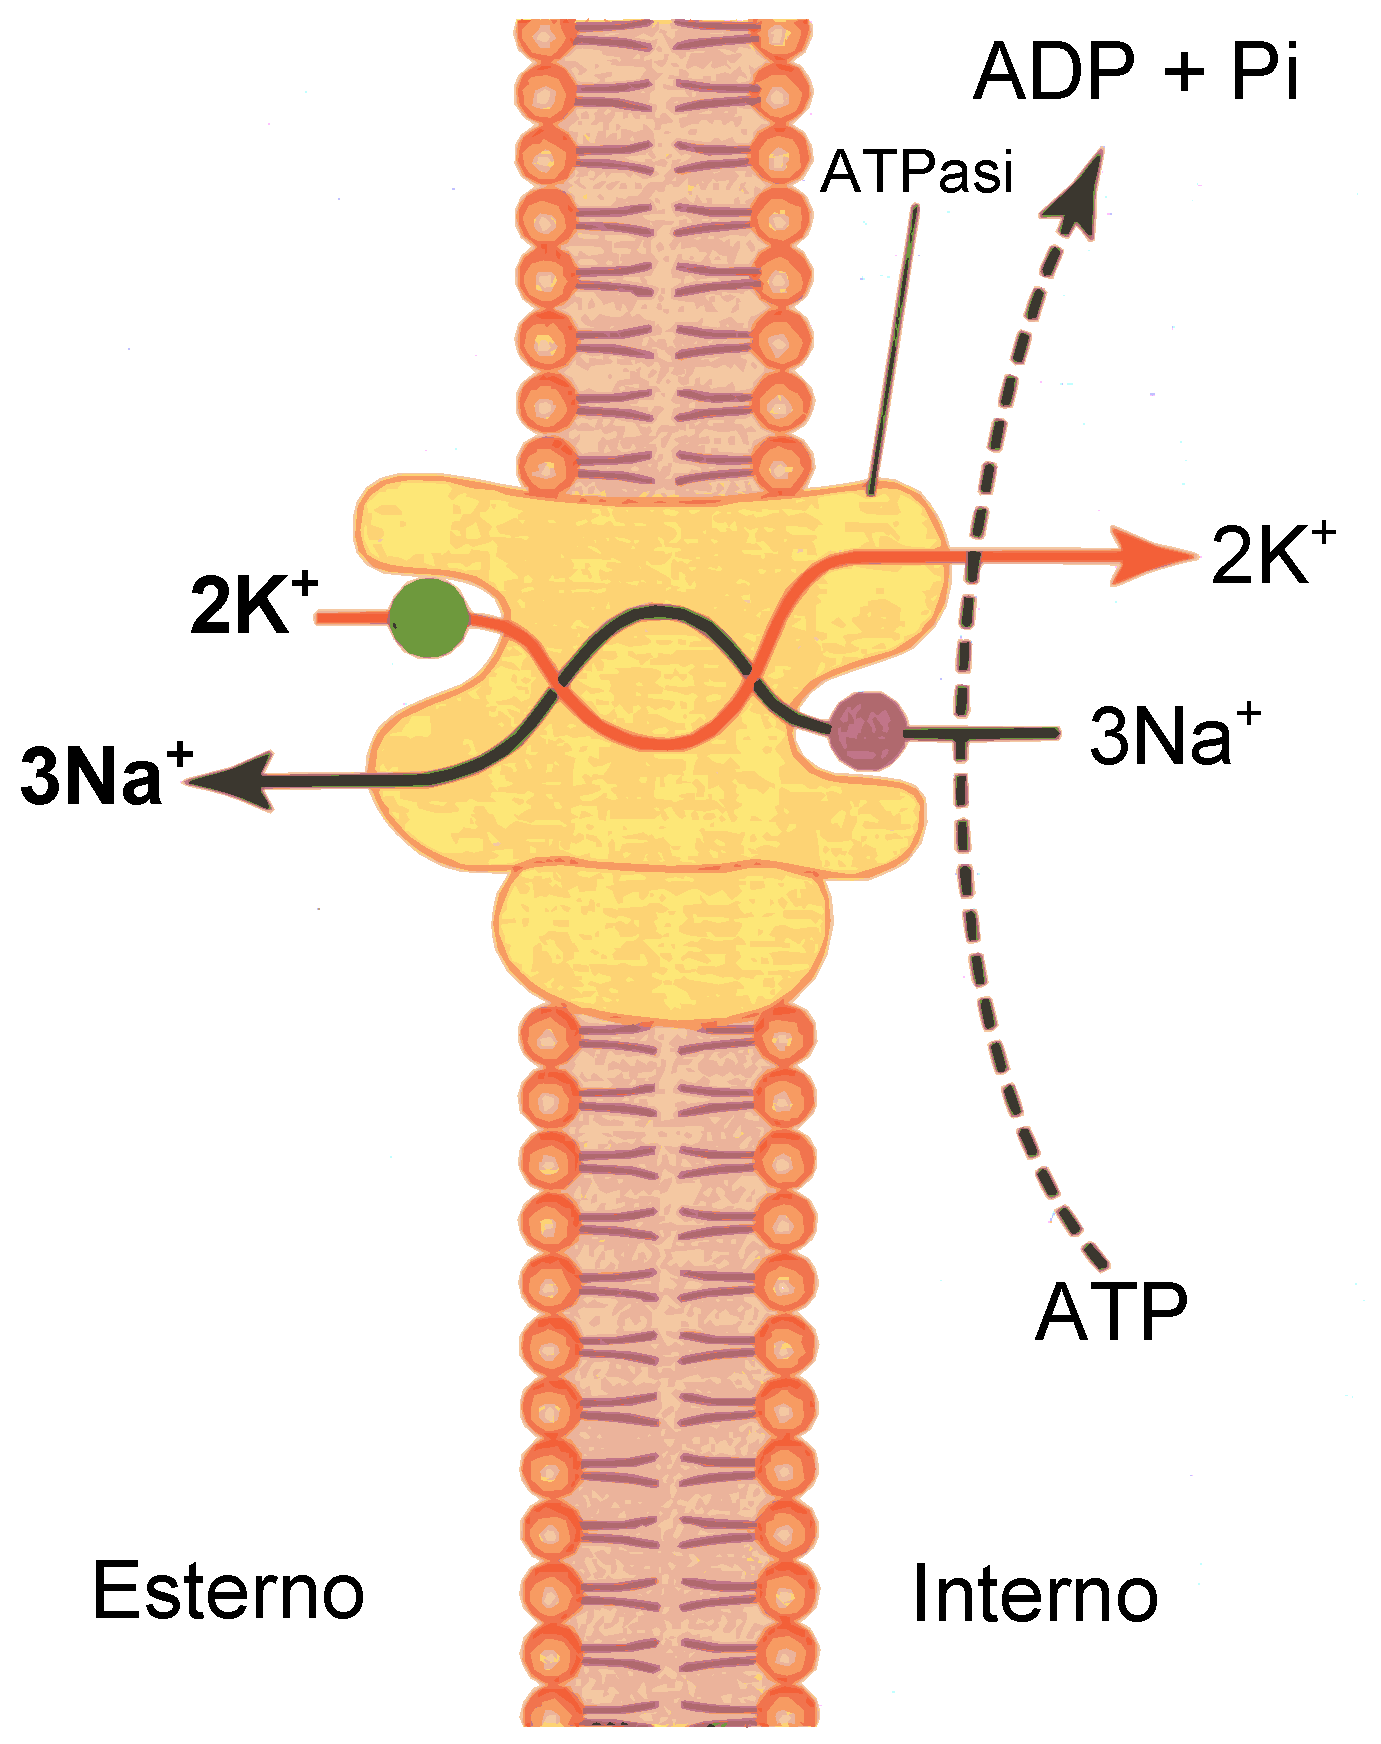
\includegraphics[width=0.4\textwidth]{immagini/atpase.eps}
  \end{center}
  \caption{Na-K~ATPasi.}\label{NaKasi}
\end{wrapfigure}

Il processo di diffusione non permette di spiegare perché alcune sostanze presentano \textit{stabilmente} alte differenze di concentrazione fra liquido extra- e intra-cellulare, come accade ad esempio per il sodio e il potassio. Poiché il processo di diffusione tenderebbe ad equilibrare le concentrazioni ai lati della membrana è plausibile che esista un meccanismo di trasporto contro-gradiente che, in condizioni stazionarie, annulli l'effetto della diffusione. Questo meccanismo è chiamato \textit{trasporto attivo} \cite{guyton}, e a differenza di quello passivo (diffusivo) impiega dell'energia, solitamente fornita dall'idrolisi dell'ATP.

Tra le sostanze che vengono trasferite mediante trasporto attivo sono compresi il sodio, il potassio, il cloro e altri ioni. Il trasporto attivo più studiato è la \textit{pompa sodio-potassio} che usa l'ATP e il cui funzionamento è illustrato in \figurename~\ref{NaKasi}. La pompa, tramite attività enzimatica, scinde l'ATP fornendo l'energia per il trasporto di tre ioni sodio all'esterno della cellula e il contemporaneo afflusso di due ioni potassio verso l'interno. Questa pompa è responsabile del mantenimento delle differenze di concentrazione di questi ioni e contribuisce a instaurare un potenziale elettrico negativo all'interno delle cellule. Ha inoltre un ruolo importante nel controllo del volume cellulare. Il controllo del volume si basa sul fatto che all'interno della cellula sono presenti molte proteine e altri composti organici che non potendo passare la membrana fosfolipidica generano una forza osmotica che richiama acqua verso l'interno della cellula e che in assenza di controllo ne provocherebbe l'esplosione. Il controllo osmotico è esercitato proprio dalla $Na^+K^+$~ATP-asi perchè il rapporto \textit{tre a due} di scambio fra gli ioni sodio e potassio equivale a una perdita netta di ioni da parte della cellula, che limita il richiamo osmotico di acqua verso l'interno. Quando per vari motivi una cellula inizia a gonfiarsi, la pompa $Na^+K^+$ aumenta la sua attività trasferendo all'esterno un numero ancora più elevato di ioni, svolgendo pertanto una continua funzione di controllo nel mantenimento del normale volume cellulare.

\subsection{Cinetica della membrana cellulare}\label{ss:trasp_membr}
Volendo ricavare una relazione quantitativa che descriva il comportamento della membrana cellulare, oltre ai meccanismi di trasporto passivo occorre tener conto anche di quelli attivi. E' possibile quindi usare la seguente equazione:\\
\begin{equation}\label{tr-att1}
	\phi_{ic} = \underbrace{k \bigl(C_{is} - C_{ic}\bigr)}_{\text{trasporto passivo}} + \underbrace{\lambda C_{is}}_{\text{trasp.attivo}}
\end{equation}
\newline
in cui si è indicato con $\phi_{ic}$ il flusso di un generico soluto verso lo spazio intracellulare ($mmol/sec$), con $k$ la velocità ($L/sec$) della diffusione, diffusione che è proporzionale alla differenza di concentrazione fra spazio interstiziale e intracellulare, e con $\lambda$ la velocità del trasporto attivo, proporzionale alla concentrazione interstiziale \cite{trasp-att}.
Introducendo il coefficiente adimensionale $\beta = (k+\lambda)/k$, è possibile riscrivere l'equazione~\ref{tr-att1} in maniera più compatta, cioè:
\begin{equation}
	\phi_{ic} = - k \bigl(C_{ic} - \beta C_{is}\bigr)
	\label{flusso_ic}
\end{equation}
Resta da chiarire con cosa si possa identificare il coefficiente $\beta$ ora introdotto. Si può osservare che in condizioni stazionarie, cioè quando ogni soluto è presente in quantità fisiologiche ai capi della membrana cellulare, trasporto passivo e attivo si bilanciano per dare un flusso netto nullo ($\phi_{ic}=0$). In questa condizione il coefficiente $\beta$ è uguale al rapporto $C_{ic,eq}/C_{is,eq}$, dove il pedice \textit{eq} sta ad indicare lo stato di equilibrio.